\documentclass[8pt,a4paper]{article}
\usepackage[utf8]{inputenc}
\usepackage{graphicx}
\graphicspath{ {./images/} }

\usepackage{color}   
\usepackage{hyperref}
\usepackage{listings}
\usepackage[utf8]{inputenc}
\usepackage{amsmath}
\usepackage{amsfonts}
\usepackage{amsthm}
\usepackage{german}

\usepackage[onehalfspacing]{setspace}


\let\stdsection\section
\setlength{\parindent}{0in} 


% Useful packages
\usepackage{amsmath}
\usepackage{graphicx}
\usepackage[colorlinks=true, allcolors=blue]{hyperref}
\title{Neuronale Netze in der Bildverarbeitung Versuch-2}
\author{Julian Schmidt MtkNr : 4705623, Vincenz Forkel MtkNr : 4097900}


\maketitle
\newpage
\begin{document}

\maketitle

\section{Einführung}

Ziel des zweiten Versuchs des Praktikums Neuronale Netze in der Bildverarbeitung im Wintersemester 2021/22 ist es Grundlagen der Bildrekonstruktion mittels Neuronaler Netze kennen zu lernen.\\
Konkret werden hierbei Ein - und Ausgänge von Multimodefasern betrachet.\\
Der Praktikumsversuch vergleicht ein Multi-Layer-Perceptron mit einem unet.\\



Hierfür wird ein Datensatz mit Bildern bestehend aus 16 mal 16 Pixeln zur Verfügung gestellt.\\



Im Verlauf des Versuches werden Probleme wie Overfitting oder zu kleine Datensätze behandelt.
\newpage

\section{Datensatz}

Zunächst wird ein Multi-Layer-Perceptron der folgenden Architektur:\\

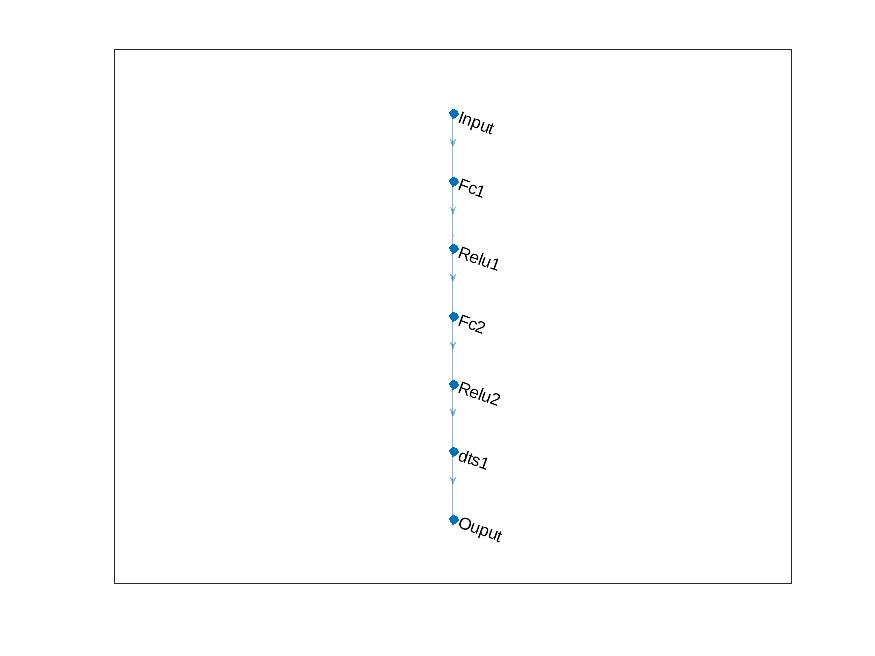
\includegraphics[scale=0.2]{layers.jpg}

\\

erstellt und mit dem gegebenem Datensatz trainiert.
Nach dem Training zeigt sich, dass die Genauigkeit des Netzes trotz Hyperparameter tuning nicht sehr hoch ist.\\
Um eine höhere Genauigkeit zu erzielen wird der Datensatz erweitert.\\
Hier werden die gegebenen Daten augmentiert.\\
Es kann Beispielsweise ein Bild leicht rotiert werden und dadurch steht ein neues Bild zur Verfügung.
Mit diesem Prinzip kann der Datensatz schnell um ein vielfaches erweitert werden.\\
Um zu untersuchen ob der erweiterte Datesatz für bessere Ergebnisse sorgt, wirds das Nets erneut trainiert, allerdings dieses mal mit dem erweitertem Datensatz.\\
Erstellt wird der Augmentierte Datensatz in dem Script create_augmented_data.m

\newpage
\subsection{Ergebnisse beider Datensätze}
Im folgendem sind verschiedene Gütekriterien in Boxplots dargestellt, um die Genauigkeit beider Netze zu bewerten.

Hierfür wird jeweils der Testdatensatz der ursprünglichen Datensatzes verwendet.\\
Es wird kein augmentierter Testdatensatz verwendet, damit für den Vergleich die gleichen Daten verwendet werden.\\

Zunächst wird der RMSE zwischen Testdatensatz und rekonstruierten Bildern beider Netze verglichen.\\

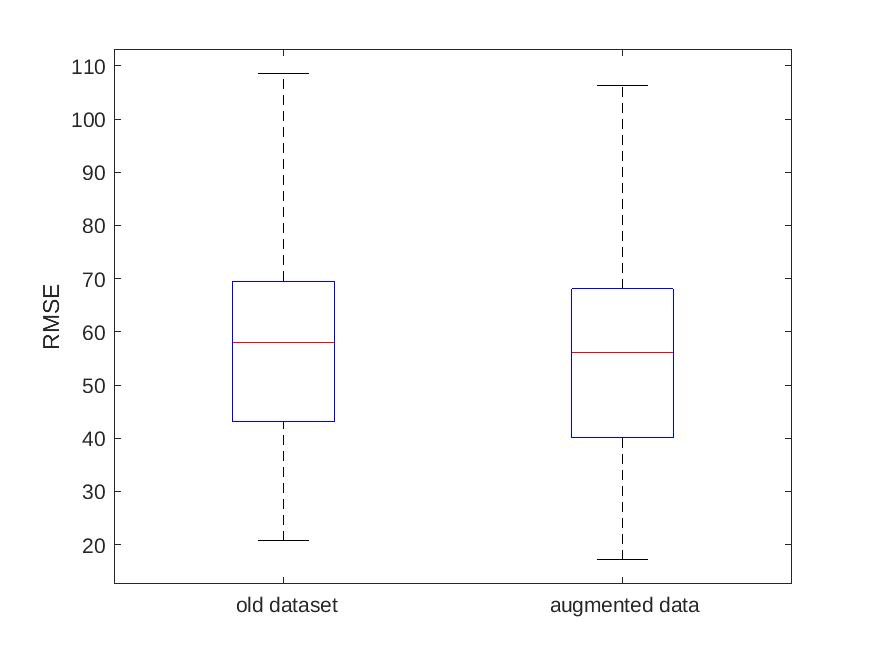
\includegraphics[scale=0.2]{boxplotRMSE.jpg}
\\
Hier zeigt sich, dass sich der RMSE beider Netze fast gleich verhält.\\
Der Interquartilsabstand des Netzes, welches mit augmentierten Daten trainiert wurde ist etwas größer.\\
Der Median ist bei beiden Netzen annährend gleich.
\\
Da die RMSEs sich sehr ähnlich sehen untersuchen wir ebenfalls die Strukturellen Ähnlichkeiten (SSIMs) der rekonstruierten Bilder

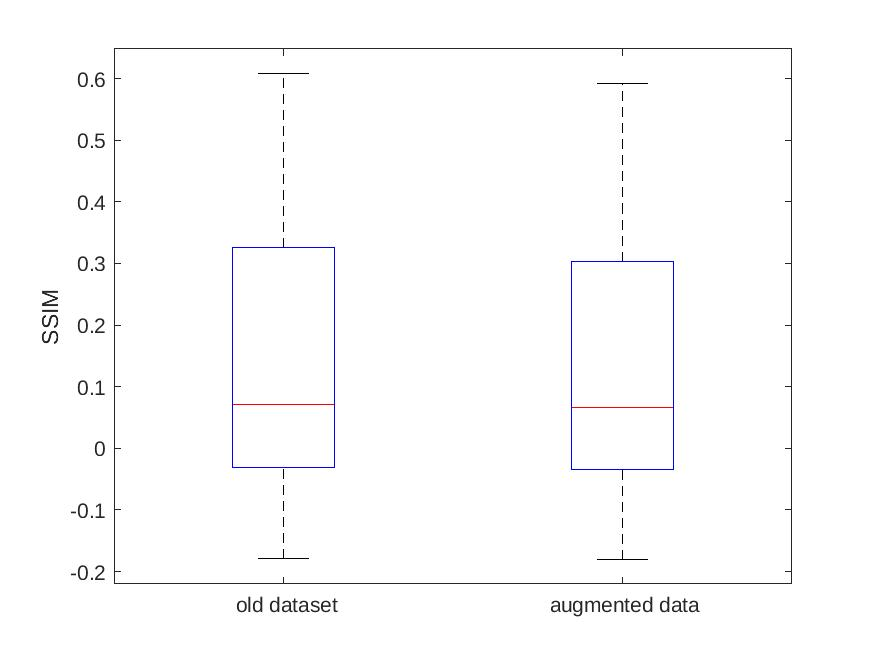
\includegraphics[scale=0.2]{boxplotSSIM.jpg}
\\
Hier zeigt sich ebenfalls das sich die rekonstruierten Bilder, beider Netze ähneln und so auch die struk. Ähnlichkeit.
Es werden ebenfalls boxplots für PSNR und Korrelationskoeffizient erstellt, diese zeigen aber ähnliches Verhalten, wie beim RMSE und SSIM.\\


\section{unet}
Da durch den augmentierten Datensatz noch keine deutliche Verbesserung erkennbar war, wird ebenfalls ein convolutional Netz trainiert.\\
Es wird das UNET verwendet.\\
Hier wird der finale convolutional Layer angepaßt.\\
Die Architektur des Netzes sieht wie folgt aus:\\
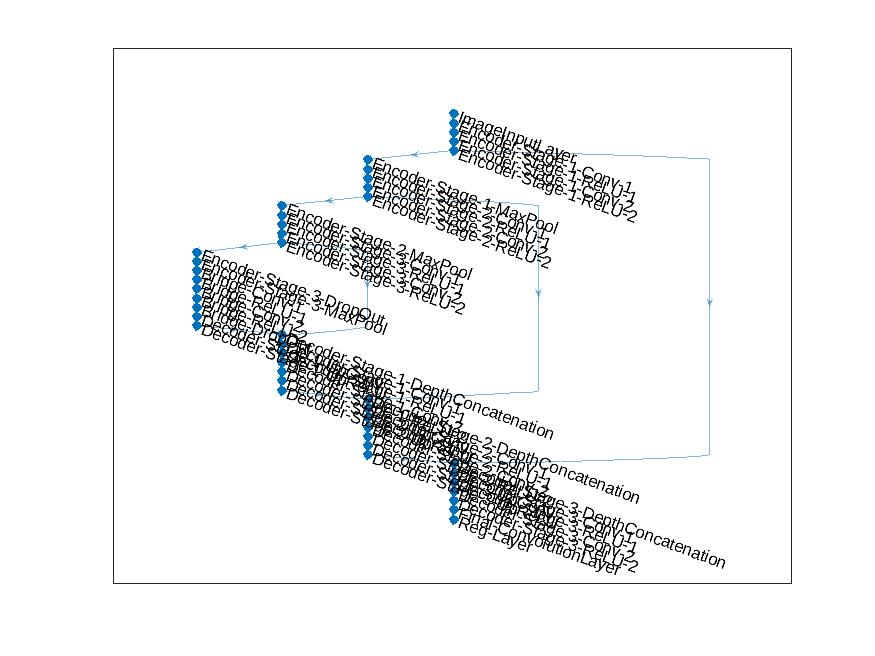
\includegraphics[scale=0.2]{unetlayers.jpg}

\subsection{Auswertung unet}
Nachdem das Unet mit dem augmentiertem Datensatz trainiert wurde wird es mit dem MLP, welches ebenfalls mit dem augmentiertem Datensatz trainiert wurde verglichen.\\
Hierzu wurden erneut die Güte Kriterien RMSE, SSIM, PSNR und Korrelationskoeffizient verwendet.\\
Es ist zuvor noch zu erwähnen, dass das unet eine deutlich höhere Zeit für das Training beansprucht, als das MLP.
Zunächst wird wieder der RMSE inspiziert.\\
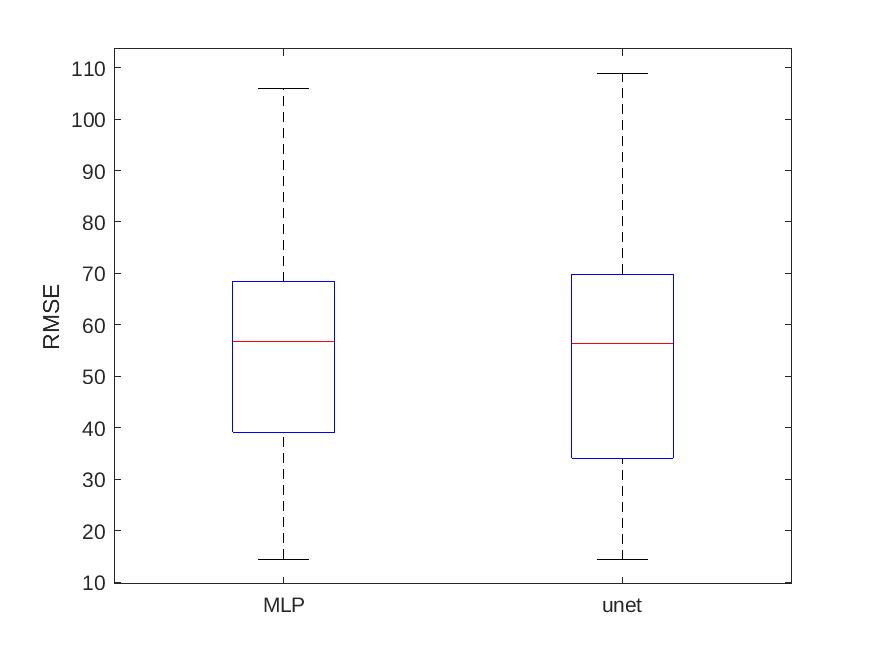
\includegraphics[scale=0.2]{boxplotUnetRMSE.jpg}


Hier zeigt sich erneut ein annährend gleiches Verhalten, der einige Unterschied ist, dass die RMSE Streuung beim unet etwas stärker ist.\\
\newpage
Um einen besseren Vergleich zu bekommen wird das SSIM ebefalls analysiert.\\

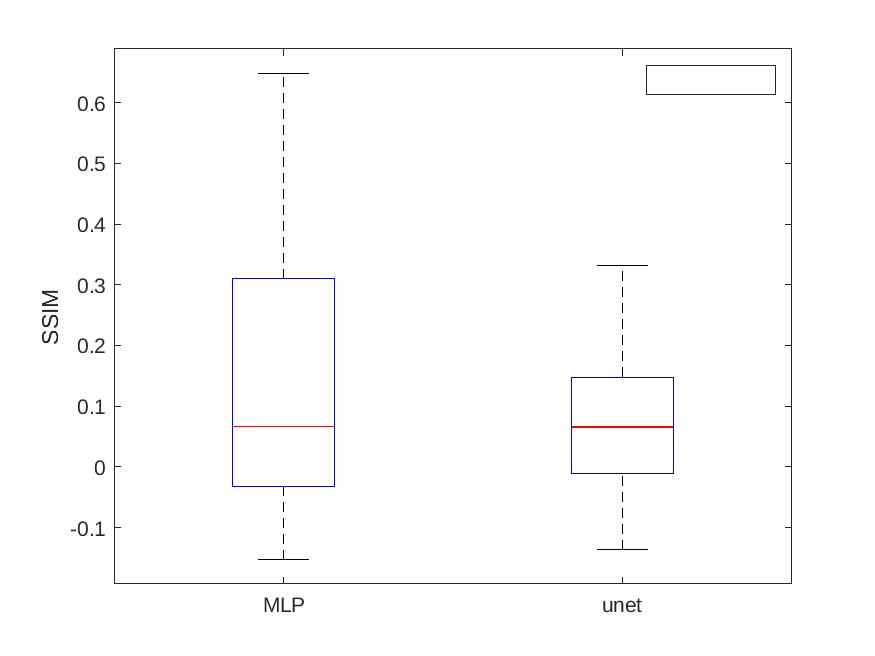
\includegraphics[scale=0.2]{boxplotUnetSSIM.jpg}

Anders als beim Vergleich beider MLPs ist dieses mal ein deutlicher Unterschied zu erkennen.
Ins Auge sticht sofort, dass der SSIM Maximalwert deutlich geringer beim unet, als beim MLP, ist.\\
Dazu ist der Interquartilsabstand ebnfalls deutlich geringer, der Median ist etwas, aber nicht deutlich, höher als beim MLP.\\

Ein annährend gleiches Verhalten ist beim PSNR zu erkennen.\\

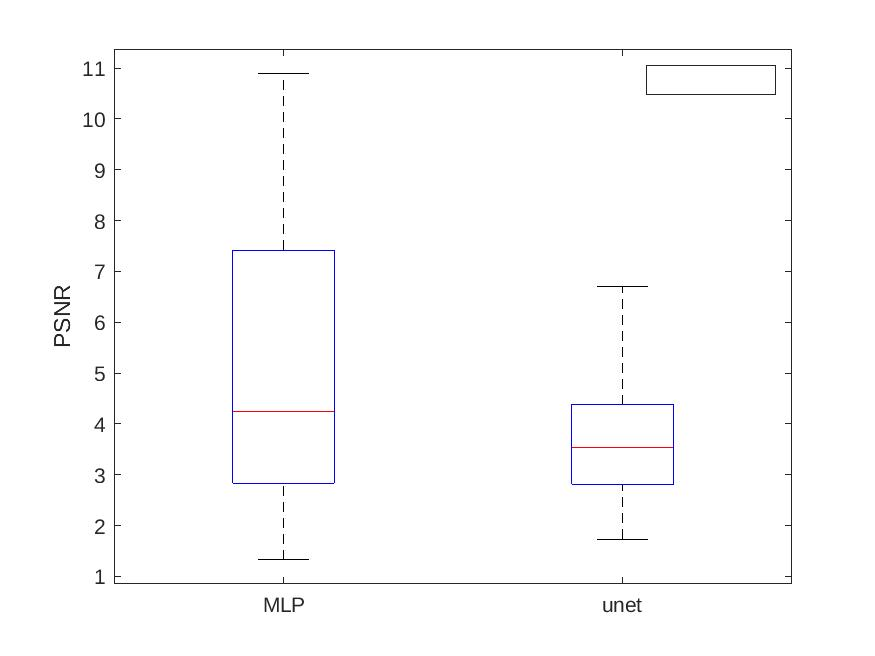
\includegraphics[scale=0.2]{boxplotUnetPSNR.jpg}\\
Der Korrelationskoeefizient hingegen verhält sich bei beiden Netzen fast gleich.\\
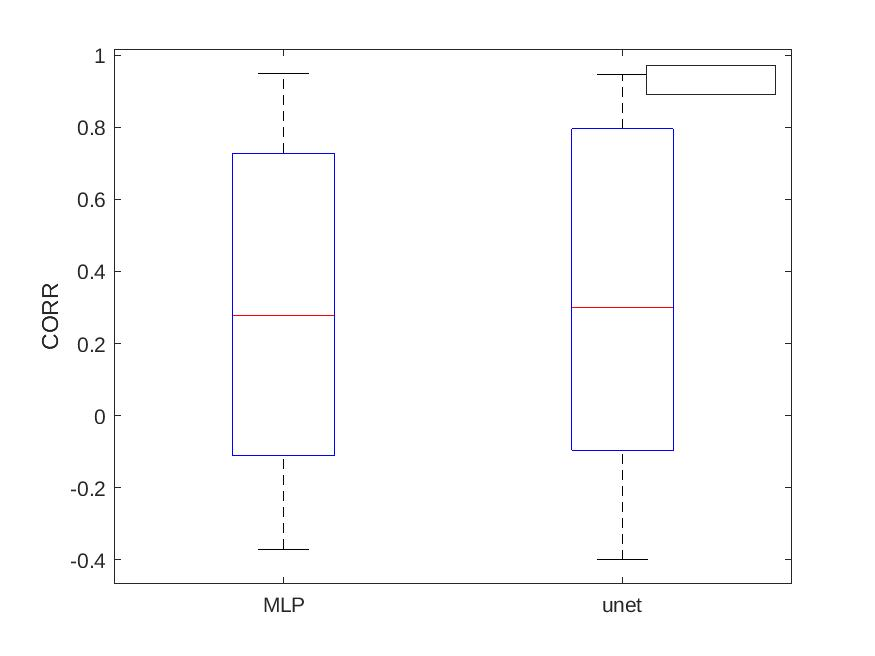
\includegraphics[scale=0.2]{boxplotUnetCORR.jpg}


\section{Trainingsverhalten}

Beim Hyperparameter-tuning der MLPS, hat sich gezeigt, dass der validation loss nach 10 Epochen leicht zu steigen beginnt, deshalb werden alle Netze mit 10 Epochen trainiert.\\
Es ist ebenfalls möglich über mehr Epochen zu trainieren und die validation patience entsprechend anzupaßen.\\
Wir konnten hiermit keinen deutlichen Perfomance Unterschied erkennen hätten uns aber etwas Zeit ersparrt, wenn wir die validation patience von Anfang an verwendet hätten, anstatt die ideale Epochen zahl von Hand zu bestimmen.\\
Die validation patience ist ein automatisierter Prozess und somit weniger Fehler anfällig, als manuelles Einstellen.\\

Abschließend ist zu sagen, dass das unet eine etwas höhere Genauigkeit erzielt, allerdings eine deutlich höhere Trainingszeit beansprucht und auch deutlich größere Rechenleistung benötigt.\\
Mit einer Leistungsfähigen GPU ist der Unterschied vermutlich deutlich geringer.\\
\end{document}
